% !TeX root = ../main.tex
% Add the above to each chapter to make compiling the PDF easier in some editors.

\chapter{Literature Review}\label{chapter:literature}
The literature review sheds light on the understanding of deepfakes, their history,
the technology driving them, the publicly available tools that create them, and
the ethical, legal, and societal issues they raise. Additionally, it examines the
countermeasures that have been developed to detect and deter them.

\section{Techniques Used in Deepfakes}\label{chapter:techniques}
Deepfakes are underpinned by significant advancements in artificial intelligence (\ac{AI})
and machine learning (ML), particularly the areas of deep learning and neural
networks. Central to the creation of deepfakes are two techniques:
Generative Adversarial Networks (\ac{GAN}s) and autoencoders.

\ac{GAN}s introduced by Goodfellow et al.~\cite{goodfellow2014generative}, nvolve two
competing neural networks: a generator and a discriminator. The generator produces
fake samples and the discriminator distinguishes between the real and fake samples.
This iterative process improves the quality of the generated samples over time as
the generator learns to create more realistic fakes to fool the discriminator. This
arms race pushes the boundaries of what \ac{GAN}s can create, contributing to the
production of deepfakes that are increasingly difficult to detect~\cite{brock2019large}.

Autoencoders, on the other hand, are a type of neural network used for learning
efficient encodings or representations of input data~\cite{doi:10.1126/science.1127647}.
In the context of deepfakes, autoencoders are used to learn the compressed
representation of faces and are then able to regenerate them based on the learned model.
The encoding of one person can be swapped with another, enabling the face of one person
to be superimposed onto another in an eerily realistic manner.

Recent developments have seen the rise of \ac{VAE} and their use in deepfake
generation~\cite{kingma2022autoencoding}. Unlike traditional autoencoders, \ac{VAE}s introduce
a probabilistic spin to the encoding and decoding processes. This allows for the
generation of new faces by sampling from the learned distribution, enhancing the
ability of the deepfake technology to generate entirely new, but convincing, faces.

\section{Publicly Available Deepfake Generation Tools}\label{chapter:publicly}
As deepfake technology has evolved, so too has the ease of access to this technology.
There are now several deepfake generation tools that are freely available and relatively
easy to use, drastically lowering the bar for entry into the world of deepfakes.

\subsection{DeepFaceLab}
Known for offering greater functionality and control over the deepfake creation
process, DeepFaceLab\footnote{\url{https://github.com/iperov/DeepFaceLab}}
has been used in several high-profile deepfake videos.
Its sophisticated technology combines the power of \ac{GAN}s and autoencoders,
leading to highly realistic face swaps in videos. DeepFaceLab offers tools
for every step of the deepfake creation process, including face extraction,
training, and video creation. This comprehensive suite of tools, combined
with its high-quality results, make it a popular choice among deepfake creators.

\begin{figure}[hb]
	\centering
	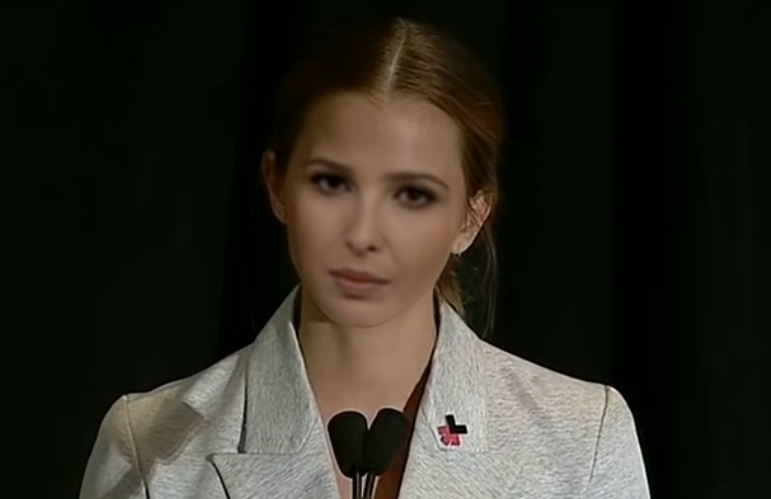
\includegraphics[scale=0.36]{figures/ivanka-deepfacelab}
	\caption{Deepfake of Ivanka Trump impersonating Emma Watson. Screenshot
		from our own generated deepfake video with DeepFaceLab.} %TODO
\end{figure}

\subsection{FaceSwap}
This community-based deepfake tool stands out with its open-source nature,
providing the user with a choice of multiple \ac{AI} models. It caters to
varying levels of experience and computing resources, making it accessible
to a wide range of users. Besides its technical merits,
FaceSwap\footnote{\url{https://faceswap.dev}} emphasizes the ethical use
of deepfake technology, warning against non-consensual use of a person's
likeness. It is more than just a tool; it's a community where people can
learn, discuss, and share knowledge about deepfakes.

\begin{figure}[ht]
	\centering
	
\includegraphics[scale=0.32]{figures/emma-stone-faceswap}
	\caption{Deepfake of Emma Stone impersonating Scarlett Johansson using
		Faceswaps's Phaze-A model. Screenshot from~\cite{emma-stone-faceswap}.}
\end{figure}

\subsection{Stable Diffuison}\label{sec:stable-diffusion}
Stable Diffusion\footnote{\url{https://stability.ai/stablediffusion}} models have
also emerged as a powerful technique for generating deepfakes.
They utilize a diffusion process to generate realistic synthetic images from a
simple Gaussian noise, achieving impressive results in the generation of
deepfake images~\cite{wu2022unifying}. One of the benefits of diffusion models
is that they can capture complex, multi-modal distributions in a way that
other generative models may struggle with. This makes them particularly
well-suited for tasks like deepfake generation, where capturing the
detailed, multi-modal distribution of human faces is essential.

\begin{figure}[ht]
	\centering
	
\includegraphics[width=0.59\columnwidth]{figures/justion-trudeau-stable-diff}
	\caption{Deepfake of Justin Trudeau created with Stable Diffusion.
		Screenshot from our own generated deepfake dataset.} %TODO
\end{figure}

\subsection{Neural Textures}
Introduced by Thies et al.~\cite{thies2019deferred}, Neural Textures represent
a method for the storage, transmission, and rendering of learned
neural representations in the context of computer graphics.
By rendering with learned features instead of geometric detail, Neural
Textures allow for more efficient representations, enabling high-quality,
photorealistic image synthesis and editing. Specifically, in the realm of
deepfakes, Neural Textures, as shown in~\autoref{fig:neural_textures}, can be trained to synthesize person-specific
details, resulting in high-quality face swaps or manipulation of facial
expressions in videos.

\begin{figure}[hb]
	\centering
	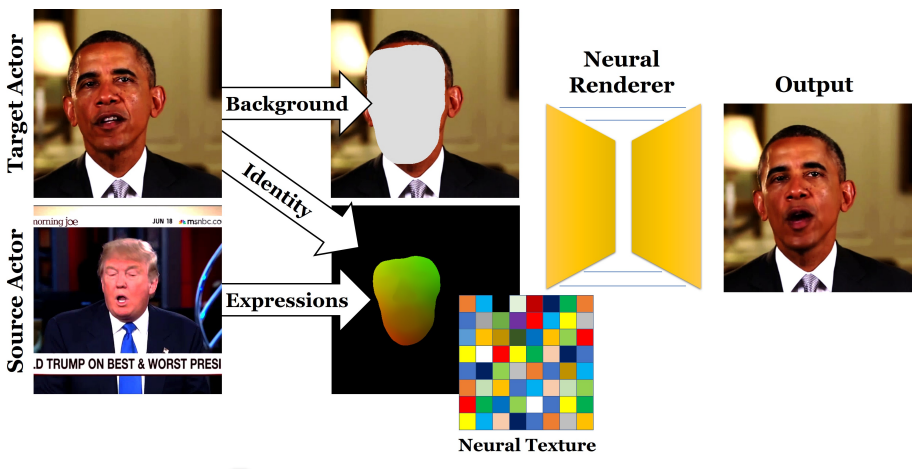
\includegraphics[width=0.7\columnwidth]{figures/neural_textures}
	\caption{The reenactment synthesis process uses expression transfer 
    to generate a UV map of the target actor that reflects the source 
    actor's expression. This map, along with a background image, is 
    processed by a neural renderer to create the final reenactment. 
    Expression alteration is achieved by training a unique neural 
    texture and renderer for the target actor, resulting in a 
    manipulated video as shown in the image from~\cite{thies2019deferred}.}\label{fig:neural_textures}
\end{figure}


\subsection{FaceApp}\label{sec:faceapp}
While not a deepfake tool in the traditional sense,
FaceApp\footnote{\url{https://www.faceapp.com/}} has gained popularity due
to its ability to transform photos of faces in various ways, such as aging,
de-aging, gender swapping, and adding smiles. The tool leverages neural
network technology for its transformations, leading to surprisingly
realistic results that have significantly contributed to the broader conversation
around the manipulation of digital imagery~\cite{faceapp}. FaceApp has
been both praised for its technological achievements and criticized for
its potential privacy and consent issues, reflecting the wider debates
surrounding the ethical implications of deepfake technology.

\begin{figure}[ht]
	\centering
	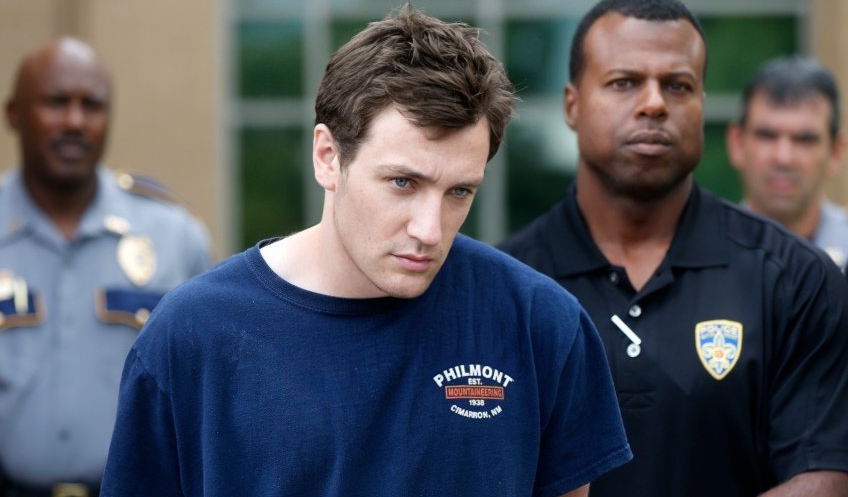
\includegraphics[width=0.61\columnwidth]{figures/faceapp}
	\caption{Deepfake created with FaceApp.} %TODO
\end{figure}


\section{Ethical and Legal Concerns}\label{chapter:legal}
The rise of deepfakes has brought with it a number of ethical and legal concerns.
At the forefront is the issue of consent, as deepfakes often involve the
use of a person's identity without their permission. This has been
particularly common in the creation of deepfake pornography, leading
to significant harm and distress for the individuals involved~\cite{chesney2019deep}.

There are also concerns about the potential misuse of deepfakes in spreading
disinformation and propaganda. Deepfakes could be used to manipulate public
opinion, interfere in elections, or even incite violence~\cite{deepfakes-business-insider,partnershiponai}.
The realistic nature of deepfakes makes it difficult for the average viewer
to distinguish truth from fake, further exacerbating these risks.

In journalism, the rise of deepfakes presents both a significant
challenge and an ethical dilemma. Journalists must not only cope with
the complex task of verifying the authenticity of deepfake content
but also think about the ethical implications of using \ac{AI}-generated
content in their reporting. Misuse of deepfakes could lead to the spread of
false information, shaking people's faith in the media~\cite{doi:10.1177/2056305120903408}.

Furthermore, the use of deepfake technology can be used to fabricate evidence in
legal cases, potentially leading to miscarriages of justice. As deepfakes become
increasingly indistinguishable from real videos, the legal system will need to
find ways to authenticate digital evidence and mitigate the risk of deepfake-generated
evidence~\cite{chesney2019deep}.

The business sector is not immune to the impact of deepfakes either. Businesses
could fall victim to deepfake scams, in which \ac{AI}-generated audio or video
is used to impersonate a company employee or other authority figure.
These scams could lead to significant financial losses or damage to a
company's reputation.

Lastly, in deepfake detection, a crucial concern is the issue of
false positives and negatives. A false positive, where a real video is wrongly
flagged as a deepfake, could have serious consequences, such as the unnecessary
spread of panic or unwarranted damage to an individual's reputation. On the
other hand, a false negative, where a deepfake is not detected and is thus
taken as genuine, can lead to the propagation of disinformation or fraud.
These challenges underscore the need for highly careful deepfake detection methods~\cite{roessler2019faceforensicspp}.

\section{Existing Countermeasures and Detection Methods}\label{chapter:countermeasures}
The rise of deepfakes demand effective countermeasures and detection methods 
to ensure information integrity and maintain public trust
in digital content. As deepfake generation techniques have become more advanced, 
detection approaches have adapted accordingly. Many of these 
approaches use machine learning, particularly deep learning techniques, 
leveraging similar technologies that power deepfakes to combat them. 

The general idea of deepfake detection is based on identifying inconsistencies
or anomalies that typically arise during the process of creating deepfakes. These
can be artifacts left by the specific algorithm used, unusual patterns in the 
distribution of the pixel values, or unnatural physical characteristics
such as inconsistent lighting or improper blinking patterns~\cite{Agarwal_2019_CVPR_Workshops}.

One approach to detect deepfakes is frequency-based analysis, where the focus is
on the differences in frequency patterns between original and deepfaked videos.
These methods, like the one proposed by Durall et al.~\cite{durall2020unmasking},
take advantage of the fact that, deepfake generation algorithms usually function in
spatial domain~\cite{spatial-domain}. As a result, they may produce distinct inconsistencies
within the frequency domain.

Another widely used approach is the \ac{CNN} based detection. This type of deep
learning model has shown excellent performance in various image and video
processing tasks due to its ability to learn hierarchical patterns in the data.
For deepfake detection, \ac{CNN}s can be trained to learn the differences between
real and fake images or videos, thus distinguishing deepfakes from the original
media~\cite{nguyen2018capsuleforensics}.

Another promising approach is the use of autoencoders for deepfake detection.
Autoencoders are a type of neural network that are trained to reconstruct
their input data. By training an autoencoder on a large amount of real face
data, it can learn to recreate real faces very well, but struggle to recreate
deepfakes, allowing the detection of deepfakes based on the reconstruction
error~\cite{cozzolino2017recasting}.

Recent advancements have led to the development of deepfake detection techniques
that analyze physiological signals. For instance, Li et al.~\cite{li2018ictu}
developed a method based on the observation that real videos contain physiological
signals that are driven by blood flow, such as heart rate. These signals, they
found, are not well preserved in synthetically generated data and thus provide
a new cue for deepfake detection.

It's important to note, however, that as deepfake generation techniques
continue to evolve, the effectiveness of these detection methods can diminish.
The constant race between deepfake creation and detection presents ongoing
challenges for researchers and developers in maintaining the efficacy of these
countermeasures.